% \knuthc  knuth the TeXBook
% \lvoc   Lvovsky
% \lamc  lamport latex 
% \slshape different font for footnote
\graphicspath{{sec01/images/s2/}{sec01/code/s2/}}
\lstset{inputpath=sec01/code/s2/}

\begin{frame}[fragile]{How good it will be if...\only<2,3>{we could write like this}}\relax
\begin{center}
\only<1>{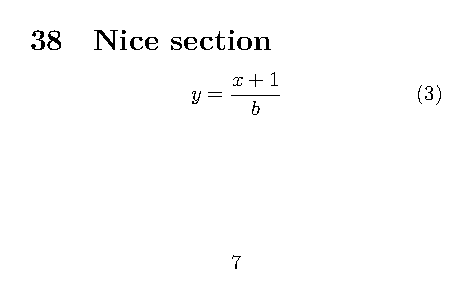
\includegraphics{refBegin}}
\only<2>{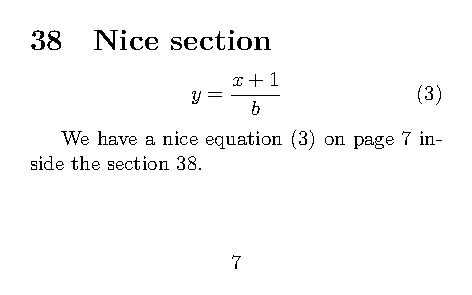
\includegraphics{refBegin2}}
\only<3>{\Huge We can!}
\end{center}

\cprotect\skfootnote{I use \verb|\only<2>{text}| for such effect. Also \verb|\setcounter| was used in source.}
\end{frame}

\begin{frame}[fragile]{Step 1: \ccol\label}\relax
    %  \lstinputlisting[linerange={12-15}]{refBegin2.tex}
     \inputminted[firstline=12, lastline=15, fontsize=\tt]{latex}{sec01/code/s2/refBegin2.tex}
     
     \skfootnote{for whole reference mechanism: \lmanc{7}[51] \lvoc{I.2.11}[27] \overC{https://www.overleaf.com/learn/latex/Cross_referencing_sections_and_equations}, \wikiC{https://en.wikibooks.org/wiki/LaTeX/Labels_and_Cross-referencing}}
\end{frame}

\begin{frame}[fragile]{Step 2: \ccol{\ref} and \ccol{\pageref}}
%, basicstyle=\tt
    %  \lstinputlisting[linerange={17-17}]{refBegin2.tex}
     \inputminted[firstline=17, lastline=17, fontsize=\tt]{latex}{sec01/code/s2/refBegin2.tex}
\end{frame}

\begin{frame}[fragile]{Combined}\relax
     \inputminted[firstline=12, lastline=17, fontsize=\tt]{latex}{sec01/code/s2/refBegin2.tex}
     
\inpause Notice \texttt{prefix\ccol{:}id} notation (\texttt{sec:nice}). It is rather common

\end{frame}

\begin{frame}[fragile]{Problem 1: lots of labels!}
    What if you have too many marks throughout the document?
    \inclasshigh{\inpause Will you have to open the .tex on the left, the .pdf on the right and compare them line by line? }
    \inpause
    
    Use package \ccol{showlabels}
\cprotect\twocolImg{
% , basicstyle=\tt\smal
    % \lstinputlisting[linerange={10-10, 13-16}]{refBeginShow.tex}
    \inputminted[firstline=10, lastline=10]{latex}{sec01/code/s2/refBeginShow.tex}
    \inputminted[firstline= 13, lastline=16]{latex}{sec01/code/s2/refBeginShow.tex}
}{refBeginShow}    
    
    
    \skfootnote{\url{http://ctan.altspu.ru/macros/latex/contrib/showlabels/showlabels.pdf}}
\end{frame}

\begin{frame}[fragile]{Problem 2: Typos}\relax
\cprotect\twocolImg{
% , basicstyle=\tt\small
    % \lstinputlisting[linerange={12-17}]{refBad.tex}
    \inputminted[firstline=12, lastline=17]{latex}{sec01/code/s2/refBad.tex}
}{refBad}

\inpause
Look at \textbf{?} in the document or inside the logs
\end{frame}

\begin{frame}[fragile]{Counter domination}\relax

look at the equation numbering style
\cprotect\twocolImg{
    \inputminted[firstline=11, lastline=19]{latex}{sec01/code/s2/refDomination.tex}
}{refDomination}

\end{frame}

\begin{frame}[fragile]{Bibliography}{How to cite}\relax
Use \ccol{\cite\{label\}}

\cprotect\twocolImg{
% , basicstyle=\tt\small
    % \lstinputlisting[linerange={9-9}]{citeFirst.tex}
    \inputminted[firstline=9, lastline=9, fontsize=\tt]{latex}{sec01/code/s2/citeFirst.tex}
}{citeFirst}  

\inpause
\cprotect\twocolImg{
% , basicstyle=\tt\small
    % \lstinputlisting[linerange={11-12}]{citeSecond.tex}
    \inputminted[firstline=11, lastline=12, fontsize=\tt]{latex}{sec01/code/s2/citeSecond.tex}
}{citeSecond}  

\skfootnote{\lmanc{8.24.2}[94] \wikiC{https://en.wikibooks.org/wiki/LaTeX/Bibliography_Management} \overC{https://www.overleaf.com/learn/latex/Bibliography_management_in_LaTeX}}     
\end{frame}

\begin{frame}[fragile]{Bibliography}{What to cite}\relax

{\csk .bib} files

\begin{verbatim}
@Book{landau,
    author = {Landau, L. D. and Lifshitz, E. M.},
    title = {The Classical Theory of Fields},
    journal = N,
    volume = {1},
    pages = {140},
    year = 1980
}
\end{verbatim}

You can have multiple records in one .bib file.
     
\end{frame}

\begin{frame}[fragile]{Offline - compile twice!}\relax
Running \LaTeX\ offline, you can get \textbf{(??)} in \ccol{\ref} and \textbf{[?]} in \ccol{\cite}. 

For 
\begin{itemize}
    \item References 
    \item Bibliography
    \item Table of content
    \item Indexing
    \item ...
\end{itemize}

\LaTeX\ collect addition data in extra files. \LaTeX\ need more then one run to get this data. 

Use \verb|latex; bibtex; latex; latex|

\inclasshigh{we will talk about the mechanism in the last lecture}

\end{frame}

\begin{frame}[fragile]{Bibliography. Where can you get .bib files?}\relax
\begin{itemize}
    \item Just google it! ``article\_name bibtex''
    \item at \url{scholar.google.ru} ask Cite -> BibTeX
    \item Go to your favorite journal and look at Citations -> ``.bib'' or ``bibtex''
    \item Ask Mendeley, Zotero or other programs to give you the .bib file
    \item Create it by yourself
\end{itemize}
\end{frame}

\begin{frame}[fragile]{Bibliography. Creating .bib file \magicPage}\relax
\begin{center}
\begin{tabular}{rl}
     \ccol{@article} & Journal or magazine article\\
\ccol{@book} & Book\\
\ccol{@conference} & Article in conference proceedings\\
\ccol{@misc} & If nothing else fits.
\end{tabular}
\end{center}

Than fill in 

{\obeylines 
\ author
\ title
\ journal
\ year
\ pages
\ volume}

following the example of other entries

\skfootnote{\wikiC{https://en.wikibooks.org/wiki/LaTeX/Bibliography_Management\#Standard_templates} for cite url checkout \stExC{https://tex.stackexchange.com/questions/3587/how-can-i-use-bibtex-to-cite-a-web-page}\\ check for full list \wikiC{https://en.wikibooks.org/wiki/LaTeX/Bibliography_Management\#BibTeX}
}     
\end{frame}

% \newcommand{\twocolImgS}[2]{  % add two columns: (1) is some text (2) is an image.
%     \begin{columns}
%         \begin{column}{0.45\textwidth}
%             #1
%         \end{column}
%         \begin{column}{0.45\textwidth}
%         \fbox{\includegraphics[width=\textwidth, keepaspectratio,page=1]{#2}}
        
%         \fbox{\includegraphics[width=\textwidth, keepaspectratio,page=2]{#2}}
%         % ниже мы делаем позиционирование, поднимая изображение на половину его высоты. Таким образом, центрированные слайды останутся центрированными и с т.з. изображения
%             % https://tex.stackexchange.com/questions/3166/how-can-the-dimensions-of-a-box-be-retrieved-with-latex
%             % \savebox{\Abox}{\includegraphics[width=\textwidth, keepaspectratio,page=1]{#2}\\\hrule\includegraphics[width=\textwidth, keepaspectratio,page=2]{#2}}
%             % \newlength{\myhh}
%             % \settoheight{\myhh}{\usebox{\Abox}}
%             % \raisebox{-0.5\myhh+1ex}[0pt][0pt]{\includegraphics[width=\textwidth, keepaspectratio,page=1]{#2}\\\hrule\includegraphics[width=\textwidth, keepaspectratio,page=2]{#2}}
%         \end{column}
%     \end{columns}
% }

% \begin{frame}[fragile]{Bibliography. Manually\magicPage}

% You can add Bibliography manually.

% \cprotect\twocolImg{
%     \inputminted[firstline=10, lastline=22]{latex}{sec01/code/s2/citeMan.tex}
%     % \lstinputlisting[linerange={10-22}]{citeMan.tex}
% }{citeMan}  

% \skfootnote{\lmanc{8.24}[92]}
% \end{frame}

% \begin{frame}[fragile]{Bibliography. Styles\magicPage}

% You can change styles.

% Mannually -- check \url{https://en.wikibooks.org/wiki/LaTeX/Bibliography_Management}

% Or with packages -- check \url{https://tex.stackexchange.com/questions/25701/bibtex-vs-biber-and-biblatex-vs-natbib}
% \end{frame}

% \begin{frame}[fragile]{Nomenclature\magicPage}\relax

%     \cprotect\twocolImg{
%         % \inputminted[firstline=9, lastline=16]{latex}{sec01/code/s2/indexmy.tex}
%         \inputminted[firstline=8, lastline=14]{latex}{sec01/code/s2/nomenclature.tex}
%     }{nomenclature}  

%     \skfootnote{\overC{https://www.overleaf.com/learn/latex/Nomenclatures}}     
% \end{frame}

% \begin{frame}[fragile]{Subject index\magicPage}\relax % предметный указатель

% \cprotect\twocolImgS{
%     \inputminted[firstline=9, lastline=16]{latex}{sec01/code/s2/indexmy.tex}
% }{indexmy}


% \skfootnote{\lvoc{IV.7}[175] \lmanc{25.2}[215]}     
% \end{frame}

